\documentclass{scrartcl}

\usepackage{amssymb}
\usepackage{amsmath}
\usepackage{tikz}

%from Negarestani - Cyclonopedia (2008), p. 36

\begin{document}
	
	%\begin{figure}
	%	\centering
	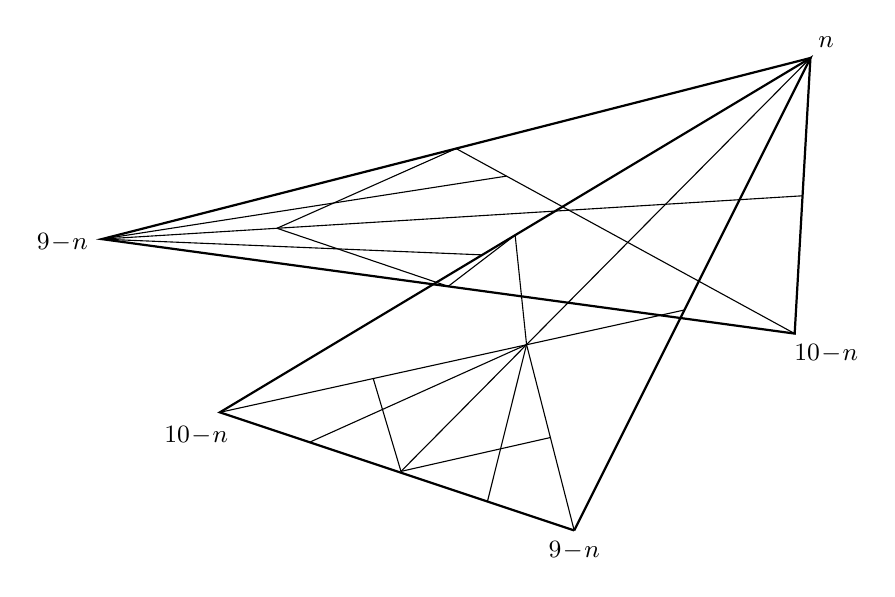
\begin{tikzpicture}
	%lower triangle
	\draw[thick] (0,0)--(-4.5,1.5)--(3,6)--(0,0);	%9-n -- 10-n -- n -- 9-n
	\node at (0,-0.25)  {\small $9\!-\!n$};
	\node at (-4.8,1.2) {\small $10\!-\!n$};
	\node at (3.2,6.2)  {\small $n$};
	\draw (-2.2,0.75)--(3,6);					%middle
	\draw (-4.5,1.5)--(1.4,2.8);				%up-right diagonal
	\draw (0,0)--(-0.605,2.36)--(-0.75,3.75);	%up-left diagonal
	\draw (-1.1,0.375)--(-0.605,2.36);
	\draw (-3.35,1.125)--(-0.605,2.36);
	%
	\draw (-2.2,0.75)--(-0.605/2,2.36/2);
	\draw (-2.2,0.75)--(-2.5525,1.93);
	
	%upper triangle
	\draw[thick] (3,6)--(2.8,2.5)--(-6,3.7)--(3,6);	%n -- 10-n -- 9-n -- n
	\draw (-6,3.7)--(2.9,4.25);					%middle
	\draw (-6,3.7)--(-1.175,3.5);
	\draw (-6,3.7)--(-0.86,4.5);
	\draw (2.8,2.5)--(-1.5,4.85);				%up-left diagonal
	\draw (-1.5,4.85)--(-3.775,3.8375);
	\draw (-1.6,3.1)--(-3.775,3.8375);
	\draw (-1.6,3.1)--(-0.75,3.75);				%only line that connects both trisons
	\node at (-6.5,3.65)  {\small $9\!-\!n$};
	\node at (3.2,2.25)  {\small $10\!-\!n$};
	\end{tikzpicture}
	%	\caption{Trison-cells generated in feedback spirals have had significant roles in presenting the Middle East as an alternative Earth dissident to the world's policies and their zeal in evolving chronologically and $t$ or environmentally relevant political approaches to the world. Parsani refers to Trison-cells as populations with sheer polytical vectors, often associated with the emergence of minorities}
	%\end{figure}
	
\end{document}